\documentclass[11pt,a4paper]{article}
\usepackage[margin=25mm]{geometry}
\usepackage[T1]{fontenc}
\usepackage[utf8]{inputenc}
\usepackage{lmodern}
\usepackage{microtype}
\usepackage{setspace}
\setstretch{1.25}
\usepackage{amsmath,amssymb}
\usepackage{graphicx}
\graphicspath{{figures/}}
\usepackage{float}
\usepackage{booktabs,tabularx}
\usepackage[font=small,labelfont=bf]{caption}
\usepackage{titlesec}
\usepackage{enumitem}
\usepackage[hidelinks]{hyperref}
\setlength{\parindent}{1em}
\setlength{\parskip}{0pt}
\setlength{\textfloatsep}{7pt plus 2pt minus 2pt}
\setlength{\floatsep}{6pt plus 2pt minus 2pt}
\setlength{\intextsep}{6pt plus 2pt minus 2pt}
\setlength{\abovedisplayskip}{5pt}
\setlength{\belowdisplayskip}{5pt}
\titlespacing*{\section}{0pt}{7pt}{3pt}
\titlespacing*{\subsection}{0pt}{5pt}{2pt}
\titleformat{\section}{\bfseries\large}{\thesection.}{0.4em}{}
\titleformat{\subsection}{\bfseries\normalsize}{\thesubsection}{0.4em}{}
\setlist{nosep,leftmargin=1.4em}

\title{\vspace{-8mm}\textbf{Compound-Truck Cross-Docking Scheduling with Arrival Time Windows:\\A Bottleneck-Guided Iterated Local Search}}
\author{Youngsoo Kim\\
\small Department of Artificial Intelligence, Yonsei University\\
\small Seoul, Republic of Korea \quad \texttt{znxkznxk1030@yonsei.ac.kr}}
\date{}

\begin{document}
\maketitle
\vspace{-5mm}

\begin{abstract}
We study a multi-door cross-dock in which a compound truck is partially
unloaded, retains one destination's freight, and then becomes that
destination's outbound carrier. Existing compound-truck models assume that
all trucks are available at time zero and minimize makespan. We introduce
known truck release times and soft departure due dates, formulate the problem
as a mixed-integer program and a CP-SAT model, and minimize makespan plus total
tardiness. Our VAA-GILS method combines a Vogel-style construction,
best-improvement descent, bottleneck-guided moves, simulated-annealing
acceptance, and kick restarts. On instances for which CP-SAT returns a
reference, GILS is within 0.1--0.6\% of its incumbents and solves a run in
0.1--2.3 seconds, versus 76--376 seconds for CP-SAT. On larger time-window
instances, GILS returns the best solutions among the tested methods. Ablations
show that descent, bottleneck moves, and restart account for the improvement;
learned operator selection does not outperform uniform sampling under equal
budgets.
\end{abstract}

\noindent\textbf{Keywords:} cross-docking; compound truck; time windows;
iterated local search; constraint programming

\section{Introduction}

Cross-docking transfers freight from inbound to outbound trucks with little
storage \cite{boysen2010,vanbelle2012}. In the compound-truck variant, one vehicle performs both roles: it
unloads freight for other destinations, retains one destination, receives that
destination's freight from other compound trucks, and departs as its carrier
\cite{joo2013,shahmardan2020}. Partial unloading can substantially shorten
makespan, but the established model assumes that all trucks are available at
time zero and has no due-date performance measure.

Release times, time windows, and tardiness are not new to conventional
cross-dock scheduling. Multi-door time-window models, ready-time models, and
mixed-service-door models have been studied in
\cite{vanbelle2013,assadi2016,bodnar2017,molavi2018,rijal2019,li2026}; uncertain or
incomplete arrivals are addressed in
\cite{larbi2011,konur2013,konurcost2013,ladier2016,xi2020}.
Those studies keep trucks purely inbound or outbound. Our contribution is to
integrate \emph{known} release times and soft due dates into the
partial-unloading compound-truck setting.

We make three contributions. First, we give MILP and CP-SAT formulations that
match an independent schedule evaluator. Second, we develop VAA-GILS, which
adds full best-improvement descent, makespan-critical and tardiness-critical
moves, and restart to the earlier VAA construction and generic neighborhoods
\cite{shahmardan2020}. Third, controlled ablations distinguish gains from the
search engine from gains due to learned operator selection. The latter does
not improve on a uniform equal-budget control in our experiments.

\section{Problem Definition}

Let $I$, $F$, $D$, $K$, and $M$ denote compound trucks, outbound trucks,
destinations, product types, and doors, respectively, with
$|I|+|F|=|D|$ and $|I|\le |M|$. Compound truck $i$ carries $f_{idk}$ units of
product $k$ for destination $d$. With unit handling time $t_k$, define
$h_{id}=\sum_k f_{idk}t_k$ and $H_i=\sum_d h_{id}$.

Each compound truck selects one retained destination and one door; at most one
compound truck uses a door. Each outbound truck selects one of the remaining
destinations and a door, and outbound trucks at the same door are sequenced.
Every destination therefore has one carrier. Truck $q\in I\cup F$ cannot start
before release time $r_q$ and has soft due date $\bar d_q$. Completion time is
$C_q$, makespan is $C_{\max}=\max_q C_q$, and tardiness is
$T_q=\max\{0,C_q-\bar d_q\}$. We minimize
\begin{equation}
 \min J=C_{\max}+\lambda\sum_{q\in I\cup F}T_q, \qquad \lambda=1.
 \label{eq:objective}
\end{equation}

Timing follows the physical sequence. If compound truck $i$ retains $d$, its
unloading completes at
$U_i=r_i+DE_i+H_i-h_{id}$. A carrier may load only after every contributing
source has finished unloading and its freight has traversed the door-to-door
transfer time. An outbound carrier must additionally wait for its release and
for the preceding occupant of its door. Loading time for destination $d$ is
$L_d=\sum_i h_{id}$; docking and undocking times are included.

\subsection{Compact MILP statement}

Binary $x_{idm}$ assigns compound truck $i$ to retained destination $d$ and
door $m$; $z_{fdm}$ analogously assigns outbound truck $f$. Let
$X_{im}=\sum_d x_{idm}$ and $Z_{fm}=\sum_d z_{fdm}$. Carrier and compound-door
assignments satisfy
\begin{align}
 \sum_{d,m}x_{idm}&=1 &&\forall i, \\
 \sum_{d,m}z_{fdm}&=1 &&\forall f, \\
 \sum_{i,m}x_{idm}+\sum_{f,m}z_{fdm}&=1 &&\forall d, \\
 \sum_{i,d}x_{idm}&\le1 &&\forall m.
\end{align}
Compound unloading is fixed by the retained destination:
\begin{equation}
 U_i=r_i+DE_i+H_i-\sum_{d,m}h_{id}x_{idm}. \label{eq:unload}
\end{equation}
Big-$M$ implications impose all incoming-transfer precedences. For example,
if $i$ carries $d$ at $m$ and source $j$ occupies $n$, then
\begin{equation}
C_i\ge U_j+t_{nm}+L_d+DL_i-B(2-x_{idm}-X_{jn}).
\label{eq:transfer}
\end{equation}
Analogous constraints set outbound start and completion times. Pairwise
precedence binaries prevent overlap between outbound trucks at the same door.
Finally, $C_{\max}\ge C_q$ and $T_q\ge C_q-\bar d_q$. The CP-SAT model replaces
big-$M$ disjunctions with enforcement literals and scales time to 0.01 units.
Fixing all assignments to a feasible schedule reproduces the independent
evaluator's completion times.

\section{VAA-GILS}

\textbf{Construction.} The VAA heuristic assigns retained destinations by
Vogel-style regret, assigns remaining destinations to outbound trucks by
completion-time priority, seeds central doors, and inserts the remaining
outbound trucks at their earliest-finishing door positions. All insertion
times enforce releases.

\textbf{Descent.} Best-improvement descent scans three move families:
outbound relocation to any door position, compound door moves/swaps, and
destination swaps between any pair of trucks. It runs on the initial solution,
on every new global incumbent, and on the final solution.

\textbf{Iterated search.} Eleven operators are available: seven generic
neighborhoods from \cite{shahmardan2020} and four guided moves. The guided
moves relocate a truck or swap a destination around either the makespan-critical
door or the most tardy truck. When no truck is tardy, the tardiness-guided moves
fall back to their makespan-critical counterparts. One operator is sampled per
iteration. A worsening candidate is accepted with probability
$\exp[-(J(s')-J(s))/T]$, with
$T_0=\max\{1,0.05J(s_0)\}$ and $T\leftarrow0.995T$.

After 30 candidate evaluations without a new best, the method restarts from
the best solution and applies three successive generic kicks, sampled
uniformly. After normal cooling, reheating applies the floor
\begin{equation}
 T\leftarrow\max\{T,0.02J(s^*)\}. \label{eq:reheat}
\end{equation}
The stagnation counters are then reset. This policy never lowers temperature
and does not necessarily return it to $T_0$.

\begin{table}[t]
\centering
\caption{Base SA-RL5 and proposed VAA-GILS.}
\label{tab:method}
\small
\begin{tabularx}{\columnwidth}{@{}lXX@{}}
\toprule
Aspect & SA-RL5 & VAA-GILS \\
\midrule
Framework & Simulated annealing & Iterated local search \\
Operators & 7 generic & 7 generic + 4 guided \\
Selection & Online tabular Q & Uniform (default) \\
Improvement & One move & Full descent \\
Stagnation & None & Kick restart + reheat \\
Objective & Makespan & Eq.~\eqref{eq:objective} \\
\bottomrule
\end{tabularx}
\end{table}

\section{Experimental Design}

We use three size regimes $(|I|,|D|,|M|)$: S $(6,9,6)$, M $(12,18,12)$,
and L $(20,30,20)$. Flows are uniform integers in $[0,20]$ for three product
types, $t_k\sim U[1,5]$, and doors lie on a random $100\times100$ layout.
Window levels are none, medium, and tight. For medium and tight windows,
$r\sim U[0,\rho H]$ and $\bar d=r+\delta H$, with
$(\rho,\delta)=(0.25,0.60)$ and $(0.50,0.35)$.

Seeds are split into disjoint train, tuning, and test pools. The main study
uses 20 independently generated test instances per cell and five stochastic
replications. We first average replications within each instance, then apply
two-sided Wilcoxon signed-rank tests to paired instance means; replications are
not treated as independent observations. GILS uses 1,000 iterations. CP-SAT
runs once per selected instance with eight threads: 300 seconds on S and 600
seconds on M/L. Only five S-none instances have proven optima; other exact
comparisons use CP-SAT incumbents.

Baselines are VAA, our implementation of SA-RL5 \cite{shahmardan2020}, and
GILS with uniform, tabular-Q, or transfer-DQN selection. The primary metric is
the per-instance gap $\Delta_{bk}$ to the best solution observed across all
methods, budgets, and CP-SAT where available.

\section{Results}

Table~\ref{tab:quality} summarizes the test results. GILS has a mean gap below
0.3\% in every cell and is within 0.1--0.6\% of CP-SAT incumbents on referenced
cells. The five S-none references are proven optimal. CP-SAT finds no feasible
schedule within 600 seconds on the larger time-window cells; there GILS
dominates the tested baselines rather than an exact reference.

\begin{table*}[t]
\centering
\caption{Mean test objective and gap to best-known solution. CP denotes the
gap to a CP-SAT reference; only S-none is proven optimal.}
\label{tab:quality}
\small
\begin{tabular}{@{}lrrrrrrrrr@{}}
\toprule
& \multicolumn{3}{c}{No windows} & \multicolumn{3}{c}{Medium} & \multicolumn{3}{c}{Tight} \\
\cmidrule(lr){2-4}\cmidrule(lr){5-7}\cmidrule(lr){8-10}
Size & VAA & GILS & $\Delta_{bk}$ & VAA & GILS & $\Delta_{bk}$ & VAA & GILS & $\Delta_{bk}$ \\
\midrule
S & 1497.5 & 1411.8 & 0.16\% & 5447.5 & 5255.7 & 0.08\% & 9276.8 & 9010.8 & 0.09\% \\
M & 3030.9 & 2928.9 & 0.29\% & 23025.5 & 22526.4 & 0.29\% & 38903.7 & 38528.0 & 0.19\% \\
L & 5492.3 & 5388.4 & 0.27\% & 55611.1 & 54846.4 & 0.10\% & 119671.9 & 118901.4 & 0.08\% \\
\bottomrule
\end{tabular}
\end{table*}

Where SA-RL5 is defined, the ordering GILS $<$ SA-RL5 $<$ VAA holds. Paired
tests show that GILS-tabular improves on VAA by 2.64\% on average
($n=180$, $p<10^{-4}$) and on SA-RL5 by 1.33\% ($n=60$, $p<10^{-4}$).
Mean GILS runtimes are 0.11, 0.52, and 2.3 seconds for S, M, and L; the
corresponding CP-SAT averages are 76, 237, and 376 seconds.

\subsection{Ablation and operator selection}

Adding makespan-critical moves to the generic pool and then adding
tardiness-critical moves improves every cell. The paired generic-to-critical
gain is 0.114 percentage points ($p<10^{-4}$); critical-to-full is 0.047
($p=0.0001$). Figure~\ref{fig:operators} shows the cell-level monotonicity.

\begin{figure}[H]
\centering
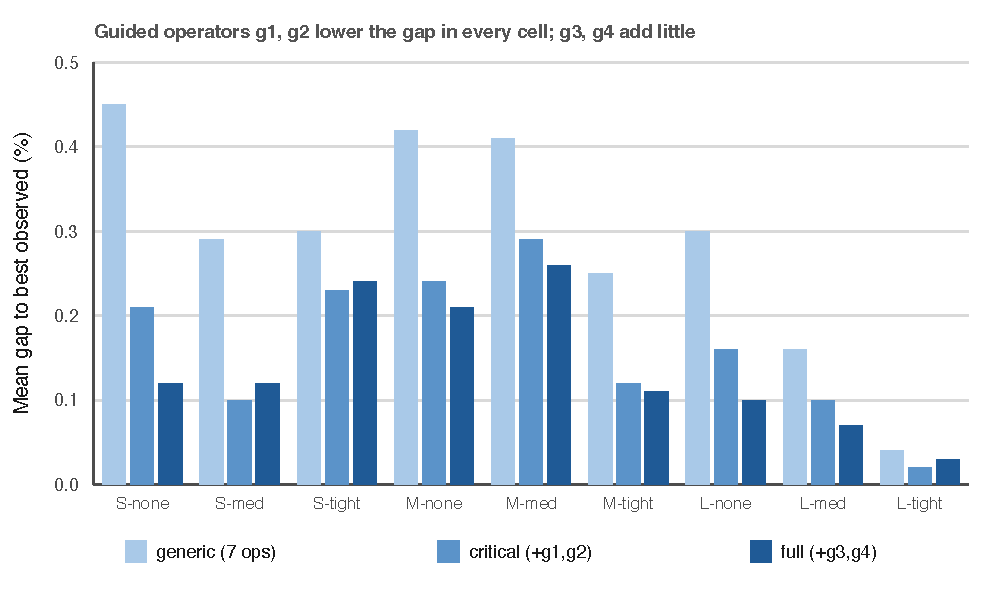
\includegraphics[width=\columnwidth]{fig2_operator_pool.pdf}
\caption{Mean gap to best-known by operator pool.}
\label{fig:operators}
\end{figure}

Leave-one-out results identify descent as the dominant component: removing it
degrades the objective by 0.156 percentage points ($p<10^{-4}$). Removing
restart costs 0.069 points ($p<10^{-4}$). VAA initialization has no detectable
pooled effect (0.022, $p=0.114$), and greedy acceptance is slightly better than
SA in this engine. Thus construction and probabilistic acceptance are not the
source of the observed performance.

\begin{figure}[H]
\centering
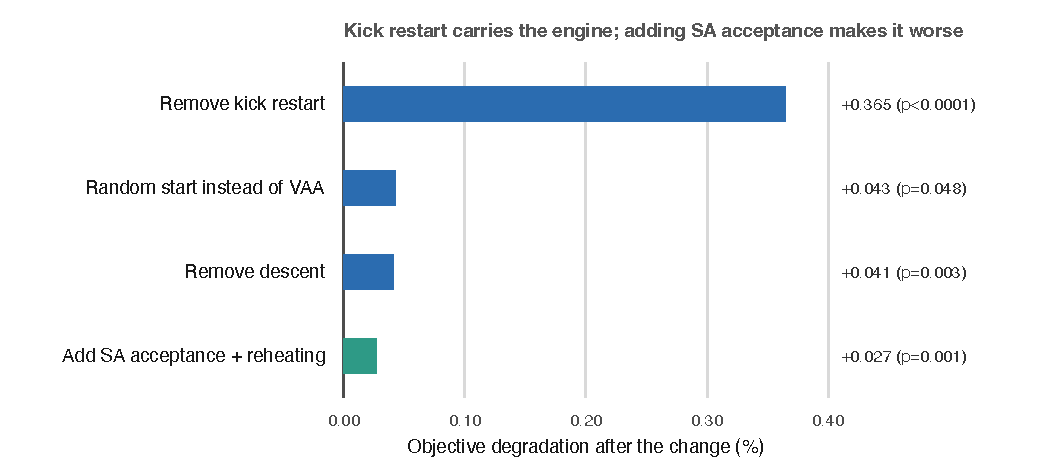
\includegraphics[width=\columnwidth]{fig3_component_ablation.pdf}
\caption{Objective degradation when a component is removed.}
\label{fig:components}
\end{figure}

Learned selection also has little incremental value. At 1,000 iterations,
tabular Q-learning differs from uniform by $-0.01$ percentage points
($p=0.150$); DQN is 0.11 points worse than uniform ($p<10^{-4}$)
\cite{watkins1992,mnih2015}. No learned
selector wins consistently over budgets of 50--3,000 iterations. This negative
result also holds on no-window cells, so it is not caused by the extension.

\begin{figure}[H]
\centering
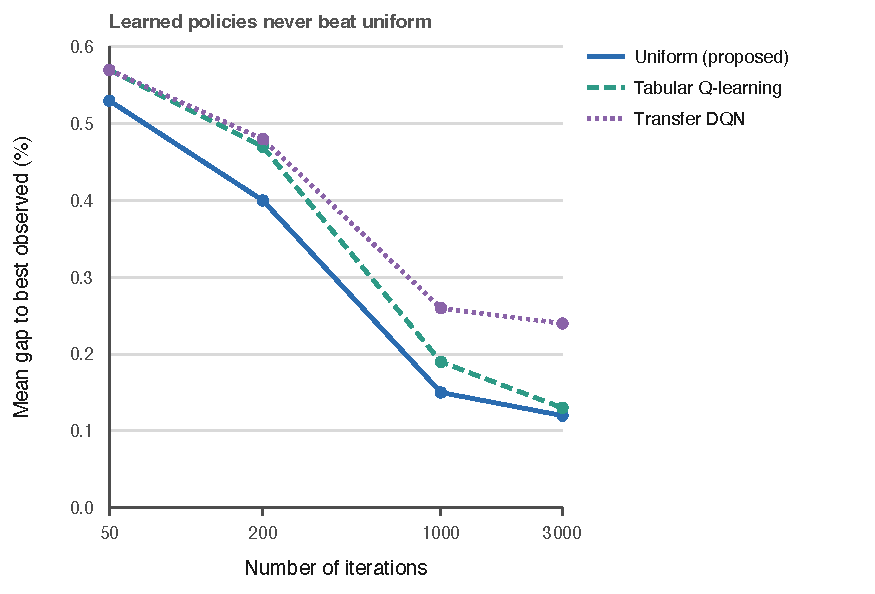
\includegraphics[width=0.72\textwidth]{fig1_selector_budget.pdf}
\caption{Mean gap to best-known across iteration budgets. The tabular selector
only edges uniform at the largest budget, while transfer DQN never wins.}
\label{fig:selector-budget}
\end{figure}

\subsection{Tardiness-weight sensitivity}

Because Eq.~\eqref{eq:objective} combines two time-valued components, we test
$\lambda\in\{0,0.25,0.5,1,2,4,8\}$ on the tuning pool. We record physical
makespan and total tardiness, min--max normalize both metrics within each
instance, and then average. Figure~\ref{fig:lambda} shows a convex trade-off.
Most tardiness reduction occurs between $\lambda=0$ and $1$, after which the
returns diminish. Across the sweep, mean makespan rises by about 1\%, whereas
mean tardiness falls by 2--3\%. We retain $\lambda=1$: it is close to the
minimum tardiness at a moderate makespan cost and gives one unit of each time
component equal weight. The sweep uses tuning rather than test instances and
is design justification, not post-hoc parameter selection.

\begin{figure}[H]
\centering
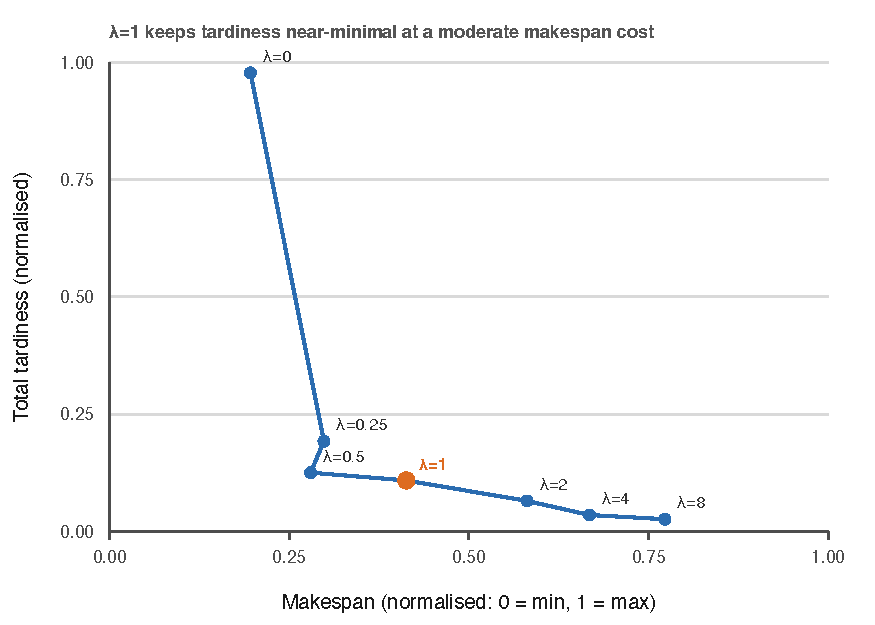
\includegraphics[width=0.72\textwidth]{fig4_lambda_tradeoff.pdf}
\caption{Normalized makespan--tardiness trade-off on tuning instances.}
\label{fig:lambda}
\end{figure}

\section{Discussion and Conclusion}

Known releases and soft due dates materially change compound-truck schedules:
carriers may wait for both source transfers and their own availability, while
door assignment couples makespan and tardiness. VAA-GILS handles this extension
quickly and approaches available CP-SAT references. Claims are deliberately
limited: only S-none has proven optima, and on large time-window cells we claim
dominance over tested baselines, not optimality.

The ablations change the interpretation of performance. Best-improvement
descent, guided moves, and restart carry the search. Once those mechanisms are
present, a uniform selector is as effective as the learned alternatives under
equal budgets. This does not imply that learning is generally ineffective;
online arrivals, heterogeneous instances, or larger operator pools may create
a stronger role for adaptation. Future work should study unrevealed arrivals,
robust schedules, tighter lower bounds, and industrial data.

\section*{Declaration of generative AI use}
During preparation, the author used OpenAI Codex (GPT-5) for language editing,
manuscript organization, bibliographic checking, and assistance in developing
and reviewing computational code. The author reviewed and verified all
references, formulations, code, results, and interpretations, and takes full
responsibility for the content.

\begin{thebibliography}{99}\small
\bibitem{assadi2016} M. T. Assadi and M. Bagheri, ``Differential evolution and
population-based simulated annealing for truck scheduling,'' \emph{Computers
\& Industrial Engineering}, vol. 96, pp. 149--161, 2016.
\bibitem{bodnar2017} P. Bodnar, R. de Koster, and K. Azadeh, ``Scheduling trucks
in a cross-dock with mixed service mode dock doors,'' \emph{Transportation
Science}, vol. 51, no. 1, pp. 112--131, 2017.
\bibitem{boysen2010} N. Boysen and M. Fliedner, ``Cross dock scheduling:
Classification, literature review and research agenda,'' \emph{Omega}, vol. 38,
pp. 413--422, 2010.
\bibitem{joo2013} C. M. Joo and B. S. Kim, ``Scheduling compound trucks in
multi-door cross-docking terminals,'' \emph{International Journal of Advanced
Manufacturing Technology}, vol. 64, pp. 977--988, 2013.
\bibitem{konur2013} D. Konur and M. M. Golias, ``Analysis of different
approaches to cross-dock truck scheduling with truck arrival time
uncertainty,'' \emph{Computers \& Industrial Engineering}, vol. 65, no. 4,
pp. 663--672, 2013.
\bibitem{konurcost2013} D. Konur and M. M. Golias, ``Cost-stable truck
scheduling at a cross-dock facility with unknown truck arrivals,''
\emph{Transportation Research Part E}, vol. 49, no. 1, pp. 71--91, 2013.
\bibitem{ladier2016} A.-L. Ladier and G. Alpan, ``Robust cross-dock scheduling
with time windows,'' \emph{Computers \& Industrial Engineering}, vol. 99,
pp. 16--28, 2016.
\bibitem{larbi2011} R. Larbi, G. Alpan, P. Baptiste, and B. Penz, ``Scheduling
cross docking operations under full, partial and no information on inbound
arrivals,'' \emph{Computers \& Operations Research}, vol. 38, no. 6,
pp. 889--900, 2011.
\bibitem{li2026} Y. Li, M. Mohammadi, X. Zhang, Y. Lan, and W. van Jaarsveld,
``Integrated trucks assignment and scheduling with mixed service mode docks,''
\emph{European Journal of Operational Research}, vol. 333, no. 1,
pp. 117--137, 2026.
\bibitem{molavi2018} D. Molavi, A. Shahmardan, and M. S. Sajadieh, ``Truck
scheduling in a cross docking systems with fixed due dates and shipment
sorting,'' \emph{Computers \& Industrial Engineering}, vol. 117, pp. 29--40,
2018.
\bibitem{rijal2019} A. Rijal, M. Bijvank, and R. de Koster, ``Integrated
scheduling and assignment of trucks at unit-load cross-dock terminals,''
\emph{European Journal of Operational Research}, vol. 278, no. 3,
pp. 752--771, 2019.
\bibitem{shahmardan2020} A. Shahmardan and M. S. Sajadieh, ``Truck scheduling
in a multi-door cross-docking center with partial unloading,'' \emph{Computers
\& Industrial Engineering}, vol. 139, Art. 106134, 2020.
\bibitem{mnih2015} V. Mnih et al., ``Human-level control through deep
reinforcement learning,'' \emph{Nature}, vol. 518, pp. 529--533, 2015.
\bibitem{vanbelle2012} J. Van Belle, P. Valckenaers, and D. Cattrysse,
``Cross-docking: State of the art,'' \emph{Omega}, vol. 40, no. 6,
pp. 827--846, 2012.
\bibitem{vanbelle2013} J. Van Belle, P. Valckenaers, G. Vanden Berghe, and
D. Cattrysse, ``A tabu search approach to the truck scheduling problem with
multiple docks and time windows,'' \emph{Computers \& Industrial Engineering},
vol. 66, no. 4, pp. 818--826, 2013.
\bibitem{watkins1992} C. J. C. H. Watkins and P. Dayan, ``Q-learning,''
\emph{Machine Learning}, vol. 8, pp. 279--292, 1992.
\bibitem{xi2020} X. Xi, C. Liu, Y. Wang, and L. H. Lee, ``Two-stage conflict
robust optimization models for cross-dock truck scheduling under uncertainty,''
\emph{Transportation Research Part E}, vol. 144, Art. 102123, 2020.
\end{thebibliography}

\end{document}
